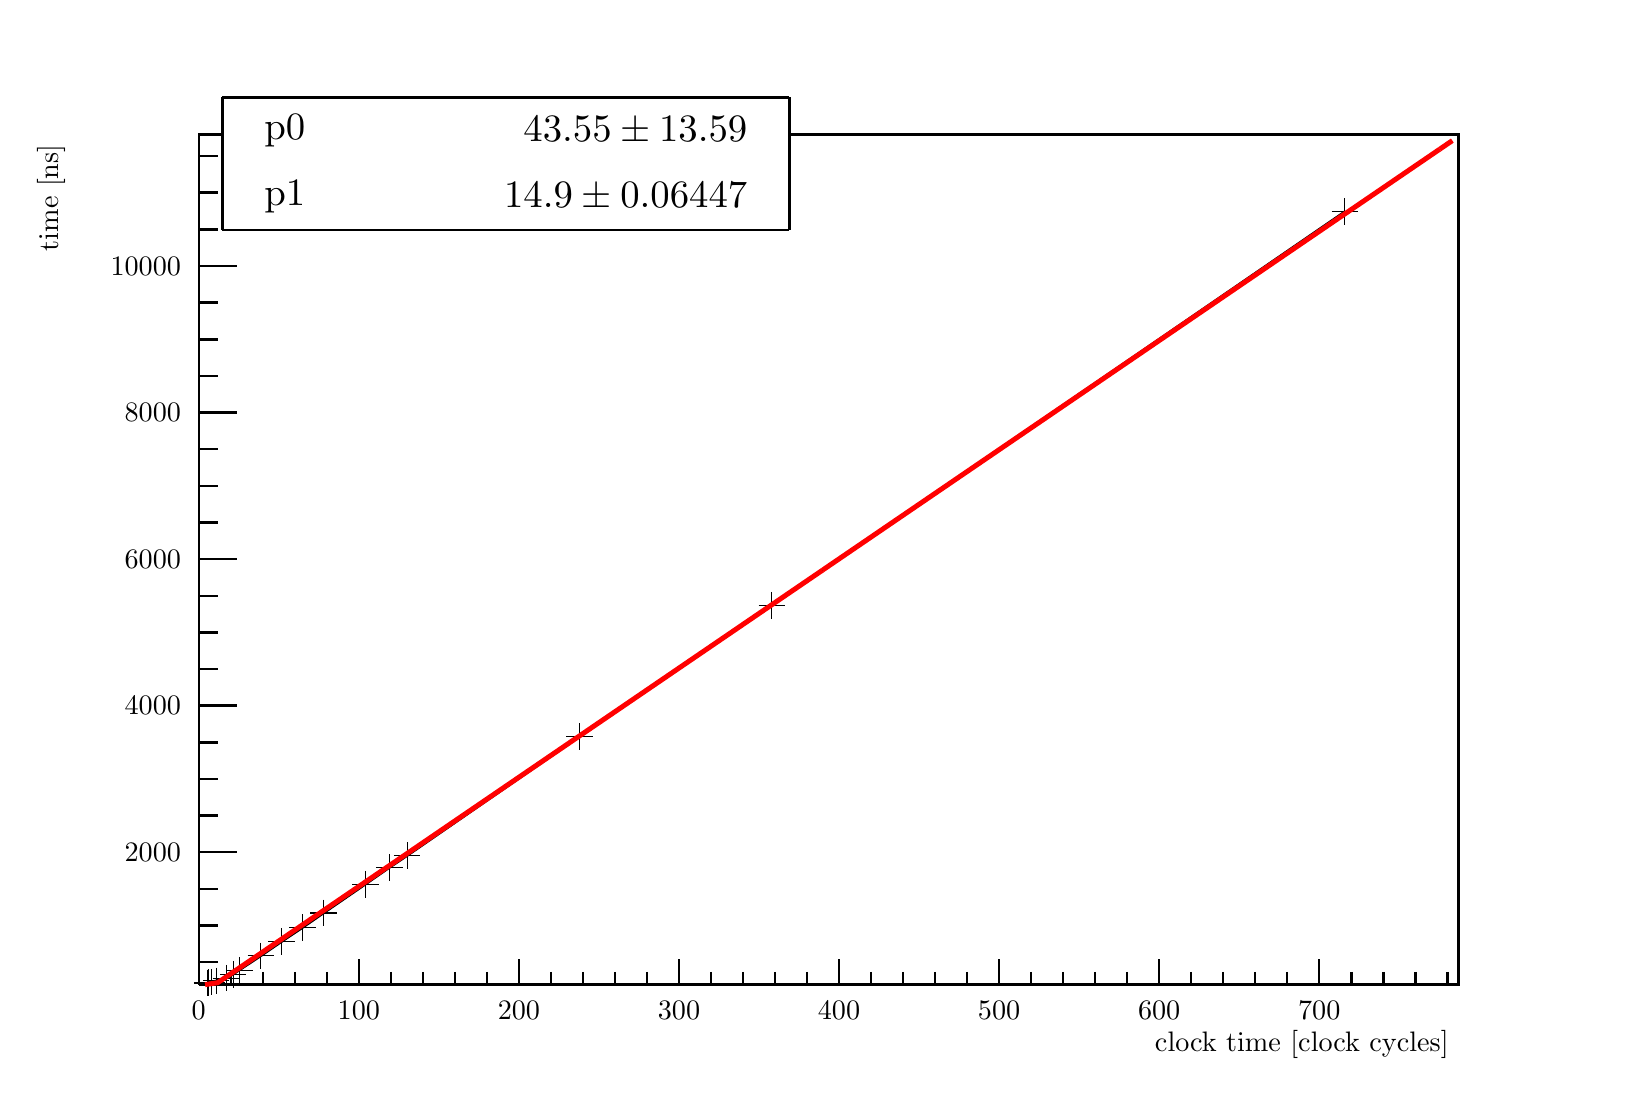
\begin{tikzpicture}
\pgfdeclareplotmark{cross} {
\pgfpathmoveto{\pgfpoint{-0.3\pgfplotmarksize}{\pgfplotmarksize}}
\pgfpathlineto{\pgfpoint{+0.3\pgfplotmarksize}{\pgfplotmarksize}}
\pgfpathlineto{\pgfpoint{+0.3\pgfplotmarksize}{0.3\pgfplotmarksize}}
\pgfpathlineto{\pgfpoint{+1\pgfplotmarksize}{0.3\pgfplotmarksize}}
\pgfpathlineto{\pgfpoint{+1\pgfplotmarksize}{-0.3\pgfplotmarksize}}
\pgfpathlineto{\pgfpoint{+0.3\pgfplotmarksize}{-0.3\pgfplotmarksize}}
\pgfpathlineto{\pgfpoint{+0.3\pgfplotmarksize}{-1.\pgfplotmarksize}}
\pgfpathlineto{\pgfpoint{-0.3\pgfplotmarksize}{-1.\pgfplotmarksize}}
\pgfpathlineto{\pgfpoint{-0.3\pgfplotmarksize}{-0.3\pgfplotmarksize}}
\pgfpathlineto{\pgfpoint{-1.\pgfplotmarksize}{-0.3\pgfplotmarksize}}
\pgfpathlineto{\pgfpoint{-1.\pgfplotmarksize}{0.3\pgfplotmarksize}}
\pgfpathlineto{\pgfpoint{-0.3\pgfplotmarksize}{0.3\pgfplotmarksize}}
\pgfpathclose
\pgfusepathqstroke
}
\pgfdeclareplotmark{cross*} {
\pgfpathmoveto{\pgfpoint{-0.3\pgfplotmarksize}{\pgfplotmarksize}}
\pgfpathlineto{\pgfpoint{+0.3\pgfplotmarksize}{\pgfplotmarksize}}
\pgfpathlineto{\pgfpoint{+0.3\pgfplotmarksize}{0.3\pgfplotmarksize}}
\pgfpathlineto{\pgfpoint{+1\pgfplotmarksize}{0.3\pgfplotmarksize}}
\pgfpathlineto{\pgfpoint{+1\pgfplotmarksize}{-0.3\pgfplotmarksize}}
\pgfpathlineto{\pgfpoint{+0.3\pgfplotmarksize}{-0.3\pgfplotmarksize}}
\pgfpathlineto{\pgfpoint{+0.3\pgfplotmarksize}{-1.\pgfplotmarksize}}
\pgfpathlineto{\pgfpoint{-0.3\pgfplotmarksize}{-1.\pgfplotmarksize}}
\pgfpathlineto{\pgfpoint{-0.3\pgfplotmarksize}{-0.3\pgfplotmarksize}}
\pgfpathlineto{\pgfpoint{-1.\pgfplotmarksize}{-0.3\pgfplotmarksize}}
\pgfpathlineto{\pgfpoint{-1.\pgfplotmarksize}{0.3\pgfplotmarksize}}
\pgfpathlineto{\pgfpoint{-0.3\pgfplotmarksize}{0.3\pgfplotmarksize}}
\pgfpathclose
\pgfusepathqfillstroke
}
\pgfdeclareplotmark{newstar} {
\pgfpathmoveto{\pgfqpoint{0pt}{\pgfplotmarksize}}
\pgfpathlineto{\pgfqpointpolar{44}{0.5\pgfplotmarksize}}
\pgfpathlineto{\pgfqpointpolar{18}{\pgfplotmarksize}}
\pgfpathlineto{\pgfqpointpolar{-20}{0.5\pgfplotmarksize}}
\pgfpathlineto{\pgfqpointpolar{-54}{\pgfplotmarksize}}
\pgfpathlineto{\pgfqpointpolar{-90}{0.5\pgfplotmarksize}}
\pgfpathlineto{\pgfqpointpolar{234}{\pgfplotmarksize}}
\pgfpathlineto{\pgfqpointpolar{198}{0.5\pgfplotmarksize}}
\pgfpathlineto{\pgfqpointpolar{162}{\pgfplotmarksize}}
\pgfpathlineto{\pgfqpointpolar{134}{0.5\pgfplotmarksize}}
\pgfpathclose
\pgfusepathqstroke
}
\pgfdeclareplotmark{newstar*} {
\pgfpathmoveto{\pgfqpoint{0pt}{\pgfplotmarksize}}
\pgfpathlineto{\pgfqpointpolar{44}{0.5\pgfplotmarksize}}
\pgfpathlineto{\pgfqpointpolar{18}{\pgfplotmarksize}}
\pgfpathlineto{\pgfqpointpolar{-20}{0.5\pgfplotmarksize}}
\pgfpathlineto{\pgfqpointpolar{-54}{\pgfplotmarksize}}
\pgfpathlineto{\pgfqpointpolar{-90}{0.5\pgfplotmarksize}}
\pgfpathlineto{\pgfqpointpolar{234}{\pgfplotmarksize}}
\pgfpathlineto{\pgfqpointpolar{198}{0.5\pgfplotmarksize}}
\pgfpathlineto{\pgfqpointpolar{162}{\pgfplotmarksize}}
\pgfpathlineto{\pgfqpointpolar{134}{0.5\pgfplotmarksize}}
\pgfpathclose
\pgfusepathqfillstroke
}
\definecolor{c}{rgb}{1,1,1};
\draw [color=c, fill=c] (0,0) rectangle (20,13.4957);
\draw [color=c, fill=c] (2,1.34957) rectangle (18,12.1461);
\definecolor{c}{rgb}{0,0,0};
\draw [c,line width=0.9] (2,1.34957) -- (2,12.1461) -- (18,12.1461) -- (18,1.34957) -- (2,1.34957);
\definecolor{c}{rgb}{1,1,1};
\draw [color=c, fill=c] (2,1.34957) rectangle (18,12.1461);
\definecolor{c}{rgb}{0,0,0};
\draw [c,line width=0.9] (2,1.34957) -- (2,12.1461) -- (18,12.1461) -- (18,1.34957) -- (2,1.34957);
\draw [c,line width=0.9] (2,1.34957) -- (18,1.34957);
\draw [c,line width=0.9] (2,1.67347) -- (2,1.34957);
\draw [c,line width=0.9] (2.40657,1.51152) -- (2.40657,1.34957);
\draw [c,line width=0.9] (2.81313,1.51152) -- (2.81313,1.34957);
\draw [c,line width=0.9] (3.2197,1.51152) -- (3.2197,1.34957);
\draw [c,line width=0.9] (3.62626,1.51152) -- (3.62626,1.34957);
\draw [c,line width=0.9] (4.03283,1.67347) -- (4.03283,1.34957);
\draw [c,line width=0.9] (4.43939,1.51152) -- (4.43939,1.34957);
\draw [c,line width=0.9] (4.84596,1.51152) -- (4.84596,1.34957);
\draw [c,line width=0.9] (5.25252,1.51152) -- (5.25252,1.34957);
\draw [c,line width=0.9] (5.65909,1.51152) -- (5.65909,1.34957);
\draw [c,line width=0.9] (6.06565,1.67347) -- (6.06565,1.34957);
\draw [c,line width=0.9] (6.47222,1.51152) -- (6.47222,1.34957);
\draw [c,line width=0.9] (6.87878,1.51152) -- (6.87878,1.34957);
\draw [c,line width=0.9] (7.28535,1.51152) -- (7.28535,1.34957);
\draw [c,line width=0.9] (7.69191,1.51152) -- (7.69191,1.34957);
\draw [c,line width=0.9] (8.09848,1.67347) -- (8.09848,1.34957);
\draw [c,line width=0.9] (8.50504,1.51152) -- (8.50504,1.34957);
\draw [c,line width=0.9] (8.91161,1.51152) -- (8.91161,1.34957);
\draw [c,line width=0.9] (9.31817,1.51152) -- (9.31817,1.34957);
\draw [c,line width=0.9] (9.72474,1.51152) -- (9.72474,1.34957);
\draw [c,line width=0.9] (10.1313,1.67347) -- (10.1313,1.34957);
\draw [c,line width=0.9] (10.5379,1.51152) -- (10.5379,1.34957);
\draw [c,line width=0.9] (10.9444,1.51152) -- (10.9444,1.34957);
\draw [c,line width=0.9] (11.351,1.51152) -- (11.351,1.34957);
\draw [c,line width=0.9] (11.7576,1.51152) -- (11.7576,1.34957);
\draw [c,line width=0.9] (12.1641,1.67347) -- (12.1641,1.34957);
\draw [c,line width=0.9] (12.5707,1.51152) -- (12.5707,1.34957);
\draw [c,line width=0.9] (12.9773,1.51152) -- (12.9773,1.34957);
\draw [c,line width=0.9] (13.3838,1.51152) -- (13.3838,1.34957);
\draw [c,line width=0.9] (13.7904,1.51152) -- (13.7904,1.34957);
\draw [c,line width=0.9] (14.197,1.67347) -- (14.197,1.34957);
\draw [c,line width=0.9] (14.6035,1.51152) -- (14.6035,1.34957);
\draw [c,line width=0.9] (15.0101,1.51152) -- (15.0101,1.34957);
\draw [c,line width=0.9] (15.4166,1.51152) -- (15.4166,1.34957);
\draw [c,line width=0.9] (15.8232,1.51152) -- (15.8232,1.34957);
\draw [c,line width=0.9] (16.2298,1.67347) -- (16.2298,1.34957);
\draw [c,line width=0.9] (16.2298,1.67347) -- (16.2298,1.34957);
\draw [c,line width=0.9] (16.6363,1.51152) -- (16.6363,1.34957);
\draw [c,line width=0.9] (17.0429,1.51152) -- (17.0429,1.34957);
\draw [c,line width=0.9] (17.4495,1.51152) -- (17.4495,1.34957);
\draw [c,line width=0.9] (17.856,1.51152) -- (17.856,1.34957);
\draw [anchor=base] (2,0.904212) node[scale=1.01821, color=c, rotate=0]{0};
\draw [anchor=base] (4.03283,0.904212) node[scale=1.01821, color=c, rotate=0]{100};
\draw [anchor=base] (6.06565,0.904212) node[scale=1.01821, color=c, rotate=0]{200};
\draw [anchor=base] (8.09848,0.904212) node[scale=1.01821, color=c, rotate=0]{300};
\draw [anchor=base] (10.1313,0.904212) node[scale=1.01821, color=c, rotate=0]{400};
\draw [anchor=base] (12.1641,0.904212) node[scale=1.01821, color=c, rotate=0]{500};
\draw [anchor=base] (14.197,0.904212) node[scale=1.01821, color=c, rotate=0]{600};
\draw [anchor=base] (16.2298,0.904212) node[scale=1.01821, color=c, rotate=0]{700};
\draw [anchor= east] (18,0.593811) node[scale=1.01821, color=c, rotate=0]{clock time [clock cycles]};
\draw [c,line width=0.9] (2,1.34957) -- (2,12.1461);
\draw [c,line width=0.9] (2.48,3.03077) -- (2,3.03077);
\draw [c,line width=0.9] (2.24,3.4961) -- (2,3.4961);
\draw [c,line width=0.9] (2.24,3.96142) -- (2,3.96142);
\draw [c,line width=0.9] (2.24,4.42674) -- (2,4.42674);
\draw [c,line width=0.9] (2.48,4.89206) -- (2,4.89206);
\draw [c,line width=0.9] (2.24,5.35738) -- (2,5.35738);
\draw [c,line width=0.9] (2.24,5.8227) -- (2,5.8227);
\draw [c,line width=0.9] (2.24,6.28802) -- (2,6.28802);
\draw [c,line width=0.9] (2.48,6.75334) -- (2,6.75334);
\draw [c,line width=0.9] (2.24,7.21866) -- (2,7.21866);
\draw [c,line width=0.9] (2.24,7.68398) -- (2,7.68398);
\draw [c,line width=0.9] (2.24,8.1493) -- (2,8.1493);
\draw [c,line width=0.9] (2.48,8.61462) -- (2,8.61462);
\draw [c,line width=0.9] (2.24,9.07995) -- (2,9.07995);
\draw [c,line width=0.9] (2.24,9.54527) -- (2,9.54527);
\draw [c,line width=0.9] (2.24,10.0106) -- (2,10.0106);
\draw [c,line width=0.9] (2.48,10.4759) -- (2,10.4759);
\draw [c,line width=0.9] (2.48,3.03077) -- (2,3.03077);
\draw [c,line width=0.9] (2.24,2.56545) -- (2,2.56545);
\draw [c,line width=0.9] (2.24,2.10013) -- (2,2.10013);
\draw [c,line width=0.9] (2.24,1.63481) -- (2,1.63481);
\draw [c,line width=0.9] (2.48,10.4759) -- (2,10.4759);
\draw [c,line width=0.9] (2.24,10.9412) -- (2,10.9412);
\draw [c,line width=0.9] (2.24,11.4066) -- (2,11.4066);
\draw [c,line width=0.9] (2.24,11.8719) -- (2,11.8719);
\draw [anchor= east] (1.9,3.03077) node[scale=1.01821, color=c, rotate=0]{2000};
\draw [anchor= east] (1.9,4.89206) node[scale=1.01821, color=c, rotate=0]{4000};
\draw [anchor= east] (1.9,6.75334) node[scale=1.01821, color=c, rotate=0]{6000};
\draw [anchor= east] (1.9,8.61462) node[scale=1.01821, color=c, rotate=0]{8000};
\draw [anchor= east] (1.9,10.4759) node[scale=1.01821, color=c, rotate=0]{10000};
\draw [anchor= east] (0.125215,12.1461) node[scale=1.01821, color=c, rotate=90]{time [ns]};
\draw [c,line width=0.9] (2.10532,1.36958) -- (2.12716,1.37423) -- (2.1596,1.38168) -- (2.21989,1.3975) -- (2.34793,1.43286) -- (2.43706,1.48126) -- (2.51357,1.53337) -- (2.78809,1.71485) -- (3.05424,1.89725) -- (3.32047,2.07594) -- (3.5858,2.25927)
 -- (4.11589,2.62408) -- (4.41906,2.83534) -- (4.64562,2.98703) -- (6.83812,4.50212) -- (9.27751,6.16797) -- (16.555,11.1664);
\foreach \P in {(2.10532,1.36958), (2.12716,1.37423), (2.1596,1.38168), (2.21989,1.3975), (2.34793,1.43286), (2.43706,1.48126), (2.51357,1.53337), (2.78809,1.71485), (3.05424,1.89725), (3.32047,2.07594), (3.5858,2.25927), (4.11589,2.62408),
 (4.41906,2.83534), (4.64562,2.98703), (6.83812,4.50212), (9.27751,6.16797), (16.555,11.1664)}{\draw[mark options={color=c,fill=c},mark size=4.804805pt,mark=+] plot coordinates {\P};}
\definecolor{c}{rgb}{1,0,0};
\draw [c,line width=1.8] (2.08,1.34957) -- (2.24,1.37372) -- (2.4,1.48284) -- (2.56,1.59197) -- (2.72,1.7011) -- (2.88,1.81023) -- (3.04,1.91936) -- (3.2,2.02849) -- (3.36,2.13762) -- (3.52,2.24675) -- (3.68,2.35588) -- (3.84,2.46501) -- (4,2.57414)
 -- (4.16,2.68327) -- (4.32,2.7924) -- (4.48,2.90152) -- (4.64,3.01065) -- (4.8,3.11978) -- (4.96,3.22891) -- (5.12,3.33804) -- (5.28,3.44717) -- (5.44,3.5563) -- (5.6,3.66543) -- (5.76,3.77456) -- (5.92,3.88369) -- (6.08,3.99282) -- (6.24,4.10195)
 -- (6.4,4.21108) -- (6.56,4.3202) -- (6.72,4.42933) -- (6.88,4.53846) -- (7.04,4.64759) -- (7.2,4.75672) -- (7.36,4.86585) -- (7.52,4.97498) -- (7.68,5.08411) -- (7.84,5.19324) -- (8,5.30237) -- (8.16,5.4115) -- (8.32,5.52063) -- (8.48,5.62976) --
 (8.64,5.73888) -- (8.8,5.84801) -- (8.96,5.95714) -- (9.12,6.06627) -- (9.28,6.1754) -- (9.44,6.28453) -- (9.6,6.39366) -- (9.76,6.50279) -- (9.92,6.61192);
\draw [c,line width=1.8] (9.92,6.61192) -- (10.08,6.72105) -- (10.24,6.83018) -- (10.4,6.93931) -- (10.56,7.04844) -- (10.72,7.15756) -- (10.88,7.26669) -- (11.04,7.37582) -- (11.2,7.48495) -- (11.36,7.59408) -- (11.52,7.70321) -- (11.68,7.81234) --
 (11.84,7.92147) -- (12,8.0306) -- (12.16,8.13973) -- (12.32,8.24886) -- (12.48,8.35799) -- (12.64,8.46712) -- (12.8,8.57624) -- (12.96,8.68537) -- (13.12,8.7945) -- (13.28,8.90363) -- (13.44,9.01276) -- (13.6,9.12189) -- (13.76,9.23102) --
 (13.92,9.34015) -- (14.08,9.44928) -- (14.24,9.55841) -- (14.4,9.66754) -- (14.56,9.77667) -- (14.72,9.88579) -- (14.88,9.99492) -- (15.04,10.1041) -- (15.2,10.2132) -- (15.36,10.3223) -- (15.52,10.4314) -- (15.68,10.5406) -- (15.84,10.6497) --
 (16,10.7588) -- (16.16,10.868) -- (16.32,10.9771) -- (16.48,11.0862) -- (16.64,11.1953) -- (16.8,11.3045) -- (16.96,11.4136) -- (17.12,11.5227) -- (17.28,11.6319) -- (17.44,11.741) -- (17.6,11.8501) -- (17.76,11.9593);
\draw [c,line width=1.8] (17.76,11.9593) -- (17.92,12.0684);
\definecolor{c}{rgb}{1,1,1};
\draw [color=c, fill=c] (2.3,10.9315) rectangle (9.5,12.6185);
\definecolor{c}{rgb}{0,0,0};
\draw [c,line width=0.9] (2.3,10.9315) -- (9.5,10.9315);
\draw [c,line width=0.9] (9.5,10.9315) -- (9.5,12.6185);
\draw [c,line width=0.9] (9.5,12.6185) -- (2.3,12.6185);
\draw [c,line width=0.9] (2.3,12.6185) -- (2.3,10.9315);
\draw [anchor= west] (2.66,12.1967) node[scale=1.40004, color=c, rotate=0]{p0       };
\draw [anchor= east] (9.14,12.1967) node[scale=1.40004, color=c, rotate=0]{$ 43.55 \pm 13.59$};
\draw [anchor= west] (2.66,11.3533) node[scale=1.40004, color=c, rotate=0]{p1       };
\draw [anchor= east] (9.14,11.3533) node[scale=1.40004, color=c, rotate=0]{$  14.9 \pm 0.06447$};
\definecolor{c}{rgb}{1,1,1};
\draw [color=c, fill=c] (2.3,10.9315) rectangle (9.5,12.6185);
\definecolor{c}{rgb}{0,0,0};
\draw [c,line width=0.9] (2.3,10.9315) -- (9.5,10.9315);
\draw [c,line width=0.9] (9.5,10.9315) -- (9.5,12.6185);
\draw [c,line width=0.9] (9.5,12.6185) -- (2.3,12.6185);
\draw [c,line width=0.9] (2.3,12.6185) -- (2.3,10.9315);
\draw [anchor= west] (2.66,12.1967) node[scale=1.40004, color=c, rotate=0]{p0       };
\draw [anchor= east] (9.14,12.1967) node[scale=1.40004, color=c, rotate=0]{$ 43.55 \pm 13.59$};
\draw [anchor= west] (2.66,11.3533) node[scale=1.40004, color=c, rotate=0]{p1       };
\draw [anchor= east] (9.14,11.3533) node[scale=1.40004, color=c, rotate=0]{$  14.9 \pm 0.06447$};
\end{tikzpicture}
